\documentclass[11pt]{article}

\usepackage[T1]{fontenc}
\usepackage[utf8]{inputenc}
\usepackage{lmodern}
\usepackage[margin=1in]{geometry}
\usepackage{microtype}
\usepackage{amsmath,amssymb,amsthm}
\usepackage{booktabs}
\usepackage{tabularx}
\usepackage{multirow}
\usepackage{xcolor}
\usepackage{listings}
\usepackage{tikz}
\usetikzlibrary{positioning,arrows.meta,fit,backgrounds,shapes.geometric}
\usepackage[numbers,sort&compress]{natbib}
\usepackage[hidelinks]{hyperref}
\usepackage{cleveref}

\hypersetup{
  pdfauthor={dgxcoder},
  pdftitle={Architecting Local, Air-Gap-Capable Desktop Clients for Agentic AI Pair Programmers}
}

\newtheorem{definition}{Definition}
\newtheorem{theorem}{Theorem}

\lstset{
  basicstyle=\ttfamily\small,
  columns=fullflexible,
  keepspaces=true,
  breaklines=true,
  frame=single,
  framerule=0.3pt,
  xleftmargin=0.5em,
  xrightmargin=0.5em,
}

\newcommand{\code}[1]{\texttt{#1}}
\newcommand{\agon}{\code{/airgapped on}}
\newcommand{\agoff}{\code{/airgapped off}}

\title{\textbf{Architecting Local, Air-Gap-Capable Desktop Clients for Agentic AI Pair Programmers: Protocol Compatibility, Process Isolation, and Host Memory Safety}}

\author{\textbf{dgxcoder}\\ \texttt{dgxcoder@dreamference.ai}}

\date{October 2026}

\begin{document}
\maketitle

\begin{abstract}
Autonomous agentic coding assistants have progressed from rudimentary terminal scripts into complex,
interactive graphical desktop environments capable of repository navigation, multi-file code synthesis,
terminal multiplexing, and background task management. However, prevailing commercial desktop clients
remain tethered to remote vendor clouds, closed model APIs, and persistent background telemetry daemons.
Deploying a vendor-free, air-gap-capable agent on modern local workstation hardware—specifically unified-memory
CPU--GPU architectures such as the NVIDIA GB10 (128\,GB unified LPDDR5X, Blackwell SM121)—presents
intricate systems challenges spanning display driver compatibility, multi-process privilege separation,
operating system sandboxing, and auditable network isolation.

In this paper, we present the architectural design, formal capability model, and empirical evaluation of
Mightling Desktop, an open-source desktop environment that speaks the same app-server protocol as the upstream
vendor's desktop client, keeps Codex-compatible defaults, runs inference on the user's own hardware, and confines
every sandboxed command to the workstation when the user turns \agon. We report five core contributions:
(1)~\textbf{A Documented Reference Point}: A description of the upstream vendor's desktop app drawn only from its
public documentation and observable behaviour, separating the open app-server protocol it drives from the window around
it, which an open client re-implements with auditable components.
(2)~\textbf{Display Subsystem Architecture}: An empirical investigation demonstrating that standard WebKitGTK
desktop wrappers fall back to CPU rasterization on NVIDIA's driver because it refuses kernel Direct
Rendering Manager (DRM) dumb buffers (\code{DRM\_IOCTL\_MODE\_CREATE\_DUMB}), causing 40--50\,ms per keystroke
frame on a $4096 \times 1700$ window; an Electron/Chromium pipeline using ANGLE over NVIDIA's own EGL/GL libraries
restores hardware compositing.
(3)~\textbf{Formal Capability Gating}: A three-tier multi-process architecture with an allowlist gatekeeper
(\code{policy.json}) over the 170-method JSON-RPC protocol, proving that no method outside the allowlist—among them
every vendor account, feedback and remote-control channel—reaches the agent from the renderer, and that the
allowlisted unconfined or networked primitives (the user's \code{!}\,command via \code{thread/shellCommand}, plugin
installs and marketplace fetches) are refused whenever \agon.
(4)~\textbf{Host Sandboxing under User-Namespace Restrictions}: A Linux sandboxing model for Ubuntu's restriction of
unprivileged user namespaces (\code{kernel.apparmor\_restrict\_unprivileged\_userns=1}) via targeted AppArmor
profiles, with no SUID root helper (\code{chrome-sandbox}) in the packaged app, and binary-level Electron fuses.
(5)~\textbf{Workstation Stability \& Audited Egress}: A two-layer host-memory safety design (a pre-load host check and
a Pressure Stall Information (PSI) watchdog) beside a resident 27B NVFP4 language model server, and an on-demand
\code{strace} egress audit that fails a session whose traced process tree reaches a non-loopback address or sends a
DNS query.
\end{abstract}

\section{Introduction}
\label{sec:intro}

The integration of Large Language Models (LLMs) into developer workflows has shifted decisively from passive
inline code completion toward autonomous agentic loops \cite{yao2023react,yang2024sweagent,wang2024openhands,jimenez2024swebench}.
Modern coding agents do not merely suggest text; they autonomously read repository structures, formulate multi-file
patches, execute build tools in local environments, parse compiler error diagnostics, and iterate until test
suites pass.

To support human-in-the-loop oversight and steering, developer interfaces have similarly evolved. Where agents
initially operated within basic Command-Line Interfaces (CLIs), developers increasingly rely on dedicated desktop
workspaces that integrate visual diff review panes, interactive terminal tabs, git worktree managers, file tree
navigators, and live artifact previewers.

Despite the release of open-source client harnesses, commercial desktop applications remain fundamentally
cloud-dependent. Commercial clients transmit repository source files, developer prompts, and tool execution
logs to remote vendor endpoints. Concurrently, background telemetry (crash reporters, metrics collectors, and
feature-flag services) keeps outbound network connections open. In sectors
governed by strict regulatory mandates—such as aerospace (ITAR), healthcare (HIPAA), financial infrastructure,
and offensive cybersecurity research—transmitting proprietary intellectual property or vulnerability exploit
code to third-party cloud infrastructure is legally prohibited or operationally unacceptable.

Deploying an autonomous coding agent entirely on-premises on a single desk-side workstation introduces
substantial systems engineering challenges that do not manifest in cloud-hosted web wrappers:
\begin{enumerate}
    \item \textbf{Display Subsystem and Driver Incompatibilities}: High-performance local AI workstations
    increasingly adopt unified CPU--GPU memory architectures (e.g., NVIDIA Blackwell GB10, Grace Hopper, Apple
    Silicon). On Linux, interactions between GPU drivers and generic webview windowing frameworks
    frequently fail, degrading interactive input performance.
    \item \textbf{Privilege Separation vs.\ Developer Capabilities}: A desktop agent client must perform high-privilege
    actions—running shell processes, inspecting git repositories, and modifying files—while ensuring that the
    webview renderer cannot be compromised by untrusted repository contents or malicious prompt injections.
    \item \textbf{Modern Kernel Sandboxing Barriers}: Contemporary Linux distributions (e.g., Ubuntu 24.04 LTS)
    restrict unprivileged user namespaces by default (via the kernel sysctl knob
    \code{apparmor\_restrict\_unprivileged\_userns}), breaking standard Chromium and container sandboxes unless
    appropriate kernel security profiles are established.
    \item \textbf{Hardware Stability under Unified Memory}: Because CPU and GPU share a common physical memory pool,
    unbounded memory growth in desktop sidecars can raise memory pressure until the host stalls or the kernel's
    Out-Of-Memory (OOM) killer ends a process, possibly the resident language model inference server.
    \item \textbf{Verifiable Egress Assurance}: Showing that no vendor channel exists, and that a strictly confined
    session stays on loopback, requires kernel-level network tracing of real sessions.
\end{enumerate}

In this paper, we describe the architecture of Mightling Desktop, an open-source, vendor-free and air-gap-capable
desktop environment built for the NVIDIA GB10 workstation. We describe the upstream vendor's desktop app from its public
documentation, detail the resolution of GPU driver rendering bottlenecks, formalize the IPC capability
gating model, and report the latency, sandboxing, and network egress results we hold records for, marking the
remaining measurements as to be made.

\paragraph{Defaults and guarantees.} Mightling follows Codex, the open-source upstream project its agent is built
from, in its defaults: at \agoff{} (the default level) sandboxed commands have the network, plugins can be installed,
the user's \code{!}\,commands run in the user's own shell, and the user may choose Full Access. Two guarantees hold
on top of that. First, at every level there is no vendor account, sign-in, telemetry or analytics channel (Mightling's
patches 0005, 0013, 0015 and 0016 to the upstream agent, checked by the egress audit of \Cref{sec:egress-audit}).
Second, at \agon{} confinement is strict: every sandboxed command runs in an empty network namespace, the host's
control sockets are masked, and Full Access and \code{!}\,commands are refused.

\subsection{Threat Model}
\label{sec:threat-model}

We assume a zero-trust threat model with respect to repository contents, visual renderer context, and network
egress:
\begin{itemize}
    \item \textbf{Threat T1: Malicious Repository / Prompt Injection.} An agent navigating a public or third-party
    repository may encounter hostile files (e.g., crafted Markdown, SVG, or HTML) designed to exploit webview
    vulnerabilities or inject malicious system prompts into the agent loop. The system must prevent renderer
    compromise from escalating to host execution.
    \item \textbf{Threat T2: Unauthorized Egress \& Exfiltration at \agon.} When the user turns \agon, untrusted
    third-party dependencies, language server extensions, or rogue model outputs must be prevented from opening
    outbound network connections, leaking source code, or performing external telemetry tracking. At \agoff{} sandboxed
    commands have the network, as in Codex, and the guarantee is the narrower one that no vendor or telemetry
    channel exists.
    \item \textbf{Threat T3: Local Privilege Escalation via SUID Helpers.} Historic browser architectures relied on SUID
    root helpers (\code{chrome-sandbox}) for process isolation. Attackers can leverage SUID binary vulnerabilities to
    achieve root privilege escalation on the developer's workstation.
    \item \textbf{Threat T4: Unified Memory Exhaustion.} An unconstrained visual client or renderer leak could exhaust
    system RAM, destabilizing the unified memory subsystem and crashing resident model inference processes.
\end{itemize}

\section{The Upstream Desktop App, from Public Material}
\label{sec:decomposition}

To fix a reference point, we describe the upstream vendor's desktop app only from its public documentation, its
release notes and what a user sees. Nothing was downloaded and unpacked, decompiled or read from the app's bundle,
and no part of it was copied; every feature Mightling offers in its place is re-implemented from that description.
Running the app was outside this study as well, because it asks for a sign-in with the vendor's account before any
surface opens.

\subsection{What the App Is}

Codex launched as a desktop app on macOS in February 2026 and on Windows in March 2026. Since July 2026 the vendor
ships it as a view inside its general desktop app, beside the vendor's other views and with its own history. The
documented platforms are macOS 14 or later, Windows on x64 and ARM64, and, as a preview since August 2026, Linux on
x64 and ARM64, installed as a \code{.deb} or \code{.rpm} package from a signed vendor package repository. The app
requires the vendor's account, and inference runs on the vendor's hosted models.

\subsection{Documented Features}

The launch announcement and the vendor's documentation and changelog describe the app as a command centre for agents:
\begin{itemize}
    \item \textbf{Projects and parallel threads}: agents run in separate threads organized by project, and the user
    switches between them without losing context. Session history and configuration are shared with the Codex CLI and
    IDE extension.
    \item \textbf{Review in the thread}: the agent's changes are reviewed as diffs (staged and unstaged, per file and
    per hunk), commented on, and opened in the user's editor.
    \item \textbf{Local and worktree modes}: a thread works in the user's checkout or in a Git worktree, and can be
    handed between the two; commit, push and pull-request creation are offered from the app.
    \item \textbf{Skills and automations}: skills are created and managed in the app and work in the CLI too;
    automations run instructions on a schedule and put their results in a review queue.
    \item \textbf{Terminal and sandbox}: an integrated terminal, and the CLI's sandbox with approval for elevated
    commands.
\end{itemize}

\subsection{The Documented Protocol}

The vendor documents app-server as the interface Codex uses to power rich clients, and it is open source in Codex's
repository \cite{openai2026codex}. It is JSON-RPC 2.0: client requests, server requests (approvals), and streamed
notifications, served over a local \code{stdio} connection to a desktop client. At the pinned release
(\code{rust-v0.158.0}) it defines 170 client request methods, 11 server request methods, 85 server notifications and 1
client notification, and \code{codex app-server generate-ts} writes TypeScript types for them. The protocol has no
commit, push, worktree or pull-request method, so a window that offers those does them itself.

\subsection{What Follows for an Open Client}

Everything that makes the desktop app a coding agent sits behind an open protocol served by an open binary. What is
the vendor's own is the window around it: its layout and interaction design, its git and terminal plumbing, and the
features tied to the vendor's account and cloud. An open client can therefore drive the same agent core, here
\code{ling app-server}, and re-implement the window from auditable components, which is what the rest of this paper
describes.

\section{Hardware and Display Architecture on Unified Memory}
\label{sec:display-hardware}

On local AI workstations featuring unified CPU--GPU memory architecture, graphics rendering performance is
inextricably coupled with kernel driver memory management.

\subsection{The WebKitGTK Dumb-Buffer Bottleneck}

Initial implementations of lightweight desktop wrappers utilized toolkits such as Tauri, which bind to system-installed
WebKitGTK (version 2.52.3 on Ubuntu 24.04). While functional for basic dialogs, typing inside an offscreen WebKitGTK
view on the NVIDIA GB10 workstation exhibited severe frame lag on a large window (\Cref{tab:keystroke-benchmarks}).

\begin{table}[t]
\centering
\small
\caption{Time per keystroke frame in an offscreen WebKitGTK 2.52.3 view on NVIDIA GB10 (driver 580.173.02; a textarea
receiving one keystroke per animation frame over 60 frames, with the app's setting \code{WEBKIT\_DISABLE\_DMABUF\_RENDERER=1}).}
\label{tab:keystroke-benchmarks}
\begin{tabularx}{\linewidth}{llrrX}
\toprule
\textbf{Toolkit} & \textbf{Window} & \textbf{Scale} & \textbf{Time per Frame} & \textbf{Compositing Path} \\
\midrule
\multirow{3}{*}{\textbf{WebKitGTK 2.52}}
  & $1280 \times 860$   & $1.0\times$  & 16\,ms & CPU Rasterization (Cairo) \\
  & $1280 \times 860$   & $2.0\times$  & 30\,ms & CPU Rasterization (Cairo) \\
  & $4096 \times 1700$  & $1.25\times$ & \textbf{40--50\,ms} & CPU Rasterization (Cairo) \\
\midrule
\textbf{Electron ANGLE} & \multicolumn{3}{l}{\textit{To be measured with the same protocol.}} & Hardware EGL / GLX \\
\bottomrule
\end{tabularx}
\end{table}

To isolate the root cause, we traced system calls made by the WebKitGTK rendering process during initialization.
With its DMABUF renderer enabled, WebKitGTK under X11 attempts to create shared Direct Rendering Manager (DRM)
``dumb buffers'' to share rendered surfaces with the display server:
\begin{lstlisting}[language=c]
ioctl(drm_fd, DRM_IOCTL_MODE_CREATE_DUMB, &args);
\end{lstlisting}
Under NVIDIA's 580.173.02 driver (open kernel modules, proprietary user-space GL/EGL), this ioctl systematically fails:
\begin{itemize}
    \item When invoked on the primary display card node (\code{/dev/dri/card1}): returns error \code{ENOSYS} (``Function not implemented'').
    \item When invoked on the render node (\code{/dev/dri/renderD128}): returns error \code{EACCES} (``Permission denied'').
\end{itemize}

The failure stems from a design difference in NVIDIA's driver: it manages framebuffers via its own memory manager
(NVKMS) and implements only part of the generic DRM interface, omitting support for the dumb-buffer ioctls on the
display node. Because WebKitGTK's one GPU path on X11 depends on DRM dumb buffers, the refusal leaves no window at all
when the DMABUF renderer is on. The app therefore ran with \code{WEBKIT\_DISABLE\_DMABUF\_RENDERER=1}, where WebKitGTK
draws with Cairo on the CPU.

\subsection{CPU Rasterization Cost Grows with Window Area}

Every setting that avoids the GPU path (DMABUF off; compositing off; compositing forced; GLX forced) lands at
40--50\,ms per keystroke frame for the $4096 \times 1700$ window, a near-full-screen window on a $5120 \times 2160$
monitor at $1.25\times$ scale: letters trail the keys at 20--25 frames per second. The default $1280 \times 860$
window stays smooth at 16\,ms, while the same window at $2\times$ scale already takes 30\,ms. The cost therefore grows
with the number of pixels the CPU must rasterize per frame. We do not attribute it to a specific bottleneck (memory
bandwidth or rasterization compute); that profile is to be measured.

\subsection{The Chromium ANGLE Hardware Pipeline}

Chromium sidesteps the DRM dumb-buffer limitation through its Almost Native Graphics Layer Engine (ANGLE) abstraction
layer. ANGLE translates WebGL and Chromium compositor draw commands into native desktop OpenGL ES, EGL, and GLX API calls.
Chromium communicates directly with NVIDIA's user-space driver libraries (\code{libEGL.so.1}, \code{libGLESv2.so.2}) and
composites directly into X11 Pixmaps, never asking for a dumb buffer. The same page in a Chromium browser on the same
machine did not lag.

By transitioning to an Electron runtime (Electron 42.11.11, pinned exactly), Mightling
Desktop restores native hardware GPU compositing on NVIDIA Blackwell hardware. Its time per keystroke frame across window
sizes, with the protocol of \Cref{tab:keystroke-benchmarks}, is to be measured.

\section{System Architecture and Process Isolation}
\label{sec:system-arch}

Mightling Desktop is structured as a three-tier multi-process architecture engineered to isolate untrusted visual
components from host operating system privileges (\Cref{fig:three-tier-arch}).

\begin{figure}[t]
\centering
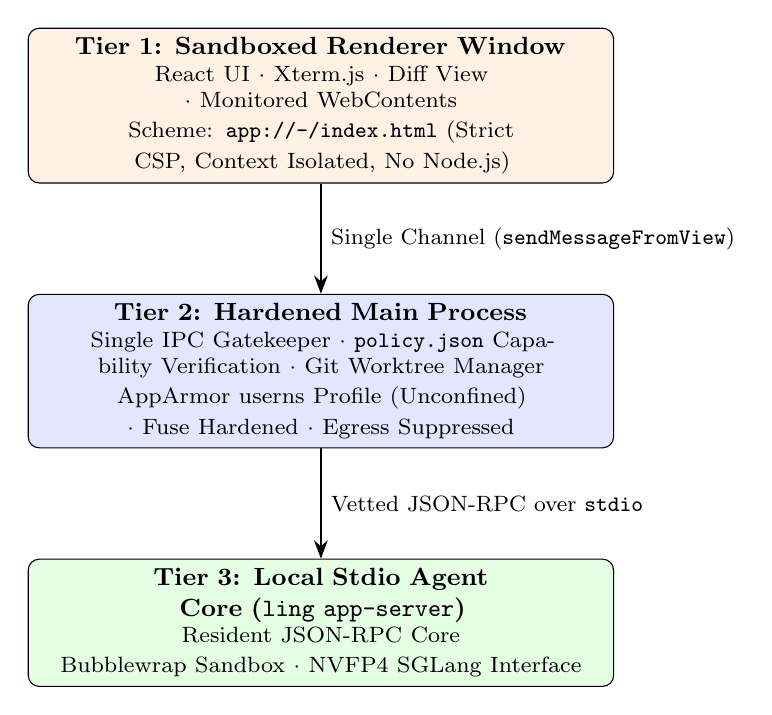
\begin{tikzpicture}[
    box/.style={draw, rounded corners, minimum height=2.4em, align=center, font=\small},
    proc/.style={box, fill=blue!10, text width=7.2cm},
    core/.style={box, fill=green!10, text width=7.2cm},
    rend/.style={box, fill=orange!10, text width=7.2cm},
    edge/.style={->, >=Stealth, thick}
]

\node[rend] (renderer) {\textbf{Tier 1: Sandboxed Renderer Window}\\
\footnotesize React UI $\cdot$ Xterm.js $\cdot$ Diff View $\cdot$ Monitored WebContents\\
\footnotesize Scheme: \code{app://-/index.html} (Strict CSP, Context Isolated, No Node.js)};

\node[proc, below=1.4cm of renderer] (main) {\textbf{Tier 2: Hardened Main Process}\\
\footnotesize Single IPC Gatekeeper $\cdot$ \code{policy.json} Capability Verification $\cdot$ Git Worktree Manager\\
\footnotesize AppArmor userns Profile (Unconfined) $\cdot$ Fuse Hardened $\cdot$ Egress Suppressed};

\node[core, below=1.4cm of main] (agent) {\textbf{Tier 3: Local Stdio Agent Core (\code{ling app-server})}\\
\footnotesize Resident JSON-RPC Core\\
\footnotesize Bubblewrap Sandbox $\cdot$ NVFP4 SGLang Interface};

\draw[edge] (renderer.south) -- node[right, font=\footnotesize] {Single Channel (\code{sendMessageFromView})} (main.north);
\draw[edge] (main.south) -- node[right, font=\footnotesize] {Vetted JSON-RPC over \code{stdio}} (agent.north);

\end{tikzpicture}
\caption{Three-tier architecture of Mightling Desktop: Sandboxed Renderer, Policy-Vetted Main Process, and Stdio Agent Core.}
\label{fig:three-tier-arch}
\end{figure}

\subsection{Tier 1: Sandboxed Renderer Window}

The visual layer is rendered within a frameless Electron window loading exclusively from a privileged custom scheme:
\code{app://-/index.html}. The scheme is registered via \code{protocol.registerSchemesAsPrivileged} with flags
\code{standard}, \code{secure}, \code{stream}, and \code{supportFetchAPI}.

To prevent cross-site scripting and unauthorized resource loading, the application delivers a strict Content Security
Policy (CSP) on all HTML responses:
\begin{lstlisting}
default-src 'none';
script-src 'self' 'wasm-unsafe-eval';
style-src 'self' 'unsafe-inline';
font-src 'self' data:;
img-src 'self' app: blob: data:;
connect-src 'self';
worker-src 'self' blob:;
base-uri 'none'; form-action 'none';
\end{lstlisting}
The renderer executes with \code{sandbox: true}, \code{contextIsolation: true}, and \code{nodeIntegration: false}.
No native filesystem or operating system APIs are injected into the DOM. The preload script exposes a minimal surface:
one messaging function, a helper that resolves a dropped file to its path, and a string naming the window type:
\begin{lstlisting}
window.electronBridge = {
  sendMessageFromView: (msg) =>   // large messages go in acknowledged pieces
    ipcRenderer.invoke("mightling_desktop:message-from-view", msg),
  pathForFile: (file) => webUtils.getPathForFile(file),
};
window.mightlingWindowType = "electron";
\end{lstlisting}

\subsection{Tier 2: Hardened Main Process Gatekeeper}

The main process acts as an immutable capability gatekeeper. It listens on the \code{mightling\_desktop:}\allowbreak\code{message-from-view}
IPC channel, with a second channel that only acknowledges the pieces of large messages. Before forwarding any request
to the underlying agent core, the main process validates the request against a compiled capability policy
(\code{policy.json}), the same file \code{ling web} enforces; both enforcers run the same conformance cases.

The main process also answers the page's own local requests—git and \code{gh}, worktrees, Night Shift, project tasks,
the \code{/airgapped} toggle and voice—each checked to come from the app window. These are not app-server methods and
lie outside the formal model of \Cref{sec:capability-gating}.

\subsection{Tier 3: The Stdio Agent Daemon}

The agent core executes as an independent, unprivileged child process:
\begin{lstlisting}[language=bash]
ling -c features.code_mode_host=true app-server
\end{lstlisting}
Communication is conducted exclusively over standard input and standard output pipes. By avoiding loopback network
sockets (e.g., \code{127.0.0.1:3000}), the architecture prevents malicious local web pages or local unprivileged
users from querying the agent daemon via standard browser \code{fetch} calls.

\section{Formal Capability Gating and Protocol Compatibility}
\label{sec:capability-gating}

The pinned upstream agent protocol (\code{rust-v0.158.0}) specifies 170 client request methods, 11 server request
methods, 85 server notifications, and 1 client notification. Rather than implementing an unconstrained proxy, Mightling
formalizes access control via a capability classification model.

\subsection{Formal Protocol Partitioning}

\begin{definition}[Protocol Universe]
Let $\mathcal{M}$ denote the universe of 170 JSON-RPC request methods defined in \code{app-server-protocol}. We define a
partition of $\mathcal{M}$ into four mutually disjoint capability tiers:
\begin{equation}
\mathcal{M} = \mathcal{T}_0 \cup \mathcal{T}_1 \cup \mathcal{T}_2 \cup \mathcal{T}_3
\end{equation}
where:
\begin{itemize}
    \item $\mathcal{T}_0$ (\textbf{Read-Only State}): Queries that inspect configuration, thread history, or models without
    mutating disk state (e.g., \code{model/list}, \code{thread/read}, \code{config/read}, \code{project/list}).
    \item $\mathcal{T}_1$ (\textbf{Confined Mutation}): Controlled mutations of threads, projects and settings
    (e.g., \code{thread/start}, \code{thread/compact/start}, \code{project/update}, \code{thread/name/set}).
    \item $\mathcal{T}_2$ (\textbf{Execution}): Execution primitives. The agent's and the terminal's commands
    (\code{command/exec}, \code{command/exec/terminate}) run under the permission profile the user picks; a
    \code{!}\,command the user types in the composer (\code{thread/shellCommand}) runs in the user's own shell.
    \item $\mathcal{T}_3$ (\textbf{Not Exposed}): Vendor and cloud channels, refused always (e.g., \code{account/login/start},
    \code{feedback/upload}, \code{remoteControl/enable}), and methods the UI does not implement, refused until reviewed.
\end{itemize}
We further distinguish $\mathcal{A} \subset \mathcal{T}_1 \cup \mathcal{T}_2$, the networked or unconfined primitives
allowed only at \agoff{}: \code{thread/shellCommand}, \code{plugin/install}, \code{marketplace/add} and
\code{marketplace/upgrade}.
\end{definition}

\begin{table}[t]
\centering
\small
\caption{Protocol capability partitioning and policy enforcement across the 170 JSON-RPC client methods.}
\label{tab:protocol-partition}
\begin{tabularx}{\linewidth}{lrXl}
\toprule
\textbf{Tier} & \textbf{Count} & \textbf{Example Methods} & \textbf{Gatekeeper Action} \\
\midrule
$\mathcal{T}_0 \cup \mathcal{T}_1 \cup \mathcal{T}_2$ (Allowed) & 73 & \code{model/list}, \code{thread/read}, \code{thread/name/set}, \code{project/update}, \code{command/exec} & Forwarded; thread openers scrubbed \\
\quad of which $\mathcal{A}$ & 4 & \code{thread/shellCommand}, \code{plugin/install}, \code{marketplace/add} & Refused at \agon \\
$\mathcal{T}_3$ (Not exposed) & 97 & \code{account/login/start}, \code{feedback/upload}, \code{remoteControl/enable} & \textbf{Rejected} (Returns $\bot$) \\
\bottomrule
\end{tabularx}
\end{table}

About a third of the 97 methods in $\mathcal{T}_3$ are vendor or cloud channels (account, feedback upload, remote
control, user verification, plugin sharing, realtime sessions). The rest are local features of the vendor's app that
Mightling's UI does not implement; the allowlist refuses them, as it refuses any method a future protocol adds, until
they are reviewed.

\begin{theorem}[Capability Containment Theorem]
Let $\mathcal{G}: \mathcal{M} \times \mathcal{P} \times \{\text{off}, \text{on}\} \to (\mathcal{M} \times \mathcal{P}) \cup \{\bot\}$
denote the capability gating function enforced by Tier 2, where $\mathcal{P}$ represents request parameters and the
third argument is the \code{/airgapped} level of the thread the request names. For every request $r = (m, p)$ at level $\ell$:
\begin{equation}
\forall m \in \mathcal{T}_3, \quad \mathcal{G}(m, p, \ell) = \bot
\qquad\text{and}\qquad
\forall m \in \mathcal{A}, \quad \mathcal{G}(m, p, \text{on}) = \bot .
\end{equation}
Furthermore, thread-opening requests (\code{thread/start}, \code{thread/resume}, \code{thread/fork}) have instruction,
provider, tool and path fields removed before delivery to Tier 3, and Ask threads are confined to a scratch folder.
Other allowed requests are forwarded unchanged; what they may do is bounded by the agent's own permission profile,
which at \agon{} refuses Full Access (patch 0023).
\end{theorem}

\begin{proof}
The gatekeeper compiles \code{ling-rs/web/policy.json} into an immutable hash set $\mathcal{S}_{\text{allowed}}$ of 73
permissible methods and a set $\mathcal{A} \subset \mathcal{S}_{\text{allowed}}$ of 4 methods refused at \agon. By construction:
\begin{equation}
\mathcal{S}_{\text{allowed}} \cap \mathcal{T}_3 = \emptyset
\end{equation}
When a message arrives at \code{mightling\_desktop:}\allowbreak\code{message-from-view}, the handler computes:
\begin{equation}
\mathcal{G}(m, p, \ell) =
\begin{cases}
(m, \text{scrub}(p)) & \text{if } m \in \mathcal{S}_{\text{allowed}} \setminus \mathcal{A}, \text{ or } m \in \mathcal{A} \text{ and } \ell = \text{off} \\
\bot & \text{otherwise}
\end{cases}
\end{equation}
where $\text{scrub}$ is the identity except on the thread openers and the configuration import. Because membership is
verified before invocation, no method in $\mathcal{T}_3$ can reach Tier 3, and no method in $\mathcal{A}$ can reach it
at \agon.
\end{proof}

\subsection{\code{thread/shellCommand}: User-Initiated, Refused at \agon}

\code{thread/shellCommand} is user-initiated: it runs a \code{!}\,command the user typed in the composer, in the
user's own shell; the agent cannot issue it. Mightling allows it while \code{/airgapped} is off, as Codex does, and
refuses it at \agon{} in both enforcers (\Cref{tab:protocol-partition}). The agent's commands run under the sandbox
mode the user picks (read-only, workspace-write or Full Access), as in Codex. Only at \agon{} does Mightling add
confinement: an empty network namespace, the host's control sockets masked, and Full Access and \code{!}\,commands
refused. Commands that need the network or host daemons fail only there.

\subsection{Prompt Injection Defense via Parameter Scrubbing}

When initiating, resuming or forking threads (\code{thread/start}, \code{thread/resume}, \code{thread/fork}), untrusted
visual extensions could attempt to inject malicious prompt overrides. The gatekeeper enforces strict parameter
scrubbing by stripping \code{droppedThreadFields}:
\begin{lstlisting}
"droppedThreadFields": [
  "baseInstructions", "developerInstructions", "modelProvider",
  "config", "personality", "dynamicTools", "environments",
  "selectedCapabilityRoots", "history", "path"
]
\end{lstlisting}
This prevents a renderer compromise from subverting the agent's core system prompt or hijacking tool capability roots.
Requests that change settings (\code{config/value/write}, \code{config/batchWrite}) and \code{command/exec} are
forwarded as sent; they act with the user's own authority, bounded by the permission profile above.

\section{Linux Host Safety and Modern Sandboxing}
\label{sec:sandboxing}

\subsection{User Namespace Restrictions in Ubuntu 24.04}

Ubuntu 24.04 LTS introduced an important kernel hardening feature:
\begin{lstlisting}
kernel.apparmor_restrict_unprivileged_userns = 1
\end{lstlisting}
When enabled, the Linux kernel refuses unprivileged calls to \code{unshare(CLONE\_NEWUSER)} or
\code{clone(..., CLONE\_NEWUSER, ...)}, returning error \code{EPERM} (``Operation not permitted'').

Historically, Chromium-based applications bypassed this restriction by installing a setuid root binary
(\code{chrome-sandbox}). However, SUID root binaries present a dangerous attack surface: vulnerabilities in SUID
helpers have historically enabled local privilege escalation to root (e.g., CVE-2016-8655, CVE-2022-2588).

\subsection{SUID-Free AppArmor Profile Integration}

The packaged Mightling Desktop ships no SUID helper. The packaging build script explicitly deletes \code{chrome-sandbox}
post-package. Instead, the \code{.deb} installs a dedicated AppArmor profile at \code{/etc/apparmor.d/mightling}:
\begin{lstlisting}
abi <abi/4.0>,
include <tunables/global>

profile mightling "/usr/lib/mightling/Mightling" flags=(unconfined) {
  userns,
  include if exists <local/mightling>
}
\end{lstlisting}
By granting the \code{userns} flag specifically to the desktop executable path, the kernel allows Chromium's multi-process
sandbox to create unprivileged user namespaces while keeping host system privileges unconfined. Development builds from
source checkouts install a development profile (\code{mightling-desktop-dev}) with \code{sudo}, so a checkout sandboxes
the same way as the Debian package. An unpacked build without \code{sudo} falls back to Chromium's setuid sandbox,
using the helper an installed Chrome, Edge or Brave provides.

\subsection{Binary Fuse Hardening}

Standard Electron binaries allow runtime inspection and arbitrary script evaluation via environment variables
(e.g., \code{ELECTRON\_RUN\_AS\_NODE=1} or \code{--inspect=9222}). To permanently disable these debug backdoors,
the packaging pipeline applies \code{@electron/fuses} v2:
\begin{itemize}
    \item \textbf{Flipped Off}:
    \code{RunAsNode},
    \code{EnableNodeOptions}\-\code{EnvironmentVariable},
    \code{EnableNodeCli}\-\code{InspectArguments}, and
    \code{GrantFileProtocol}\-\code{ExtraPrivileges}.
    \item \textbf{Flipped On}:
    \code{EnableCookieEncryption},
    \code{EnableEmbeddedAsar}\-\code{IntegrityValidation},
    \code{OnlyLoadAppFromAsar}, and
    \code{WasmTrapHandlers}.
\end{itemize}
These fuses mutate binary bits in the compiled ELF executable, so Node's run-as-node, \code{NODE\_OPTIONS} and inspect
hooks are disabled in the binary even if an attacker controls environment variables. Chromium's own command-line switches,
such as \code{--remote-debugging-port}, are not fuses and are outside this guarantee.

\section{Workstation Memory Stability on Unified Hardware}
\label{sec:memory-stability}

On unified-memory architectures like the NVIDIA GB10, host CPU RAM and GPU VRAM reside on the same physical
128\,GB LPDDR5X bus. When serving a 27B-parameter language model (Qwen3.8-27B in NVFP4) with a block diffusion drafter
via SGLang, the weights take about 20\,GB; SGLang's static share (memory fraction 0.50) holds them and the KV pool, and
about 39\,GB of host memory stays available while serving. A timeline of memory residency over a long session (model,
KV pool and desktop client) is to be measured.

On unified memory, a model load can freeze the whole host. Mightling guards it with two layers: \code{check\_host\_safety()}
refuses a load on a host that is not safe, and a watchdog (\code{MemoryPressureWatchdog}) follows Linux Pressure Stall
Information (PSI) during the load and stops the model container, through the fastest kill path the host can still run,
before the host stalls. Once the model is resident, a leaking visual client could still raise memory pressure until the
kernel's OOM killer ends a process, possibly the model server. Mightling Desktop bounds its own memory via three rules:
\begin{enumerate}
    \item \textbf{Single-Process Daemon}: Every window—the main one, new windows, pop-outs, and detached terminal and
    diff panes—multiplexes over a single resident \code{ling app-server} daemon, eliminating multi-instance process
    duplication.
    \item \textbf{Cache Evacuation in Development}: When the app is run from a checkout (\code{ling-admin desktop run}),
    Chromium's HTTP cache directory (\code{Cache/}) is purged at start; the packaged app and \code{ling app} keep
    Chromium's default cache.
    \item \textbf{Bounded Async Operations}: Filesystem access to the user's folders times out after 10 seconds, and
    \code{git} and \code{gh} output is capped at 16\,MB, so large directory trees and outputs cannot exhaust the heap.
\end{enumerate}

\section{On-Demand Network Egress Auditing}
\label{sec:egress-audit}

To verify that the desktop application opens no vendor channel and that its session stays on loopback, Mightling
incorporates an automated kernel-level egress audit (\code{ling-admin audit egress --app}).

\subsection{Audit Methodology}

The egress auditor runs the packaged desktop application with hidden windows, in an isolated scratch environment, for a
40-second session under system call tracing; \code{ling-admin codex build} runs the audit too:
\begin{lstlisting}[language=bash]
strace -f -e trace=connect,sendto,sendmsg,sendmmsg,execve,write,writev
\end{lstlisting}
The audit monitors every socket creation, destination IP address, and payload transmission. Crucially, tracing
\code{sendmmsg} captures asynchronous DNS queries issued by \code{glibc}. It judges the traced \code{ling} or app
process tree against loopback. Services outside that tree reach the internet by design at \agoff: the SearXNG
container behind loopback port 8888, which queries search engines for \code{ling-search}, and any messenger bridge
the user turned on, which the audit names as a declared exception rather than failing it.

\begin{table}[t]
\centering
\small
\caption{What the audited session may reach. At \agoff{} the web-search container and enabled messenger bridges,
outside the traced process tree, are named exceptions.}
\label{tab:egress-verification}
\begin{tabularx}{\linewidth}{lllX}
\toprule
\textbf{Destination Port} & \textbf{Binding} & \textbf{Protocol} & \textbf{Authorized Service} \\
\midrule
Configured model port & \code{127.0.0.1} & HTTP/JSON & Local SGLang / vLLM model inference server. \\
Port 8767 & \code{127.0.0.1} & HTTP/JSON & Local read-only Gmail sidecar. \\
Port 8768 & \code{127.0.0.1} & HTTP/JSON & Local image search service. \\
Port 8888 & \code{127.0.0.1} & HTTP/JSON & Local SearXNG web search engine. \\
\midrule
\textbf{Disallowed Ports} & \textbf{Any} & \textbf{Any} & \textbf{Audit Verdict: FAIL} \\
Port 53 (DNS) & External & UDP/TCP & Prohibited (no DNS query may leave the traced tree). \\
All External IPs & Non-Loopback & TCP/UDP & Prohibited for the traced process tree. \\
\bottomrule
\end{tabularx}
\end{table}

\subsection{Egress Suppression in Renderer Previews}

When rendering live HTML previews, web pages frequently attempt background network calls via DNS prefetching:
\begin{lstlisting}
<link rel="dns-prefetch" href="//telemetry.example.com">
\end{lstlisting}
Testing revealed that the Chromium Blink renderer resolves DNS prefetch links directly from the renderer process,
bypassing standard Electron web request filters. To neutralize this leak, the desktop application initializes with:
\begin{itemize}
    \item \code{--blink-settings=dnsPrefetchingEnabled=false}
    \item Custom response header: \code{X-DNS-Prefetch-Control: off}
    \item Command-line switches: \code{--disable-background-networking}, \code{--disable-component-update}.
\end{itemize}
The audit's app session passes only if the traced process tree makes no non-loopback connection and sends no DNS
query (\Cref{tab:egress-verification}).

\section{Cross-Platform Architectures: macOS and Windows on Arm}
\label{sec:cross-platform}

While Linux on NVIDIA Blackwell represents the primary deployment platform for local model workstations,
extending the desktop pair-programming architecture to developer laptops (such as Apple Silicon macOS and Windows 11
on Arm PCs) exposes distinct platform-specific systems constraints.

\subsection{macOS Pipeline: Metal Compositing and TCC Filesystem Gates}

On macOS (Apple Silicon M-series unified memory architectures), the graphics subsystem differs fundamentally from Linux X11:
\begin{enumerate}
    \item \textbf{Metal Rendering Pipeline}: Rather than translating through OpenGL ES or Vulkan, Chromium ANGLE maps directly
    to Apple's Metal API framework. This delivers hardware compositing without the dumb-buffer allocation failures observed under
    Linux X11 drivers; frame timing on macOS is to be measured.
    \item \textbf{Transparency, Consent, and Control (TCC) Deadlocks}: macOS enforces strict sandbox consent via the TCC subsystem.
    The first programmatic filesystem access to sensitive developer directories (\code{\~/Documents}, \code{\~/Desktop}, or \code{\~/Downloads})
    triggers an interactive system dialog. In preliminary builds, executing synchronous directory walks (\code{fs.readdirSync}) during
    startup blocked the main \code{libuv} event loop while awaiting user consent. This induced an unrecoverable windowless freeze where
    teardown failed to respond even to \code{SIGTERM}. Mightling Desktop resolves this by mandating asynchronous non-blocking walks
    (\code{fs.promises}) governed by bounded 10-second timeouts.
    \item \textbf{Keychain Subsystem Mocking}: On ad-hoc signed or development preview builds, Chromium's \code{os\_crypt} framework
    queries the macOS Keychain (``Mightling Safe Storage'') via \code{SecItemCopyMatching}, hanging the process if an unlocked login
    keychain is unavailable. Because the app holds no vendor credentials and talks to its agent over local pipes, the application
    launches with \code{--use-mock-keychain}, completely eliminating interactive keychain prompts.
\end{enumerate}

\subsection{Windows 11 on Arm: Direct3D ANGLE and the Agent's Windows Sandbox (Preview)}

The desktop app has no released Windows build. This subsection records the design for Windows 11 on Arm (targeting
Snapdragon X Elite and NVIDIA N1X developer workstations) and says which parts exist in code:
\begin{enumerate}
    \item \textbf{Direct3D Compositing via DXGI}: On Windows, Chromium binds ANGLE to Direct3D 11 via the DirectX Graphics
    Infrastructure (DXGI), so the driver-level dumb-buffer issue does not arise; frame timing is to be measured.
    \item \textbf{Codex's Windows Sandbox at \agon}: Without Linux network namespaces, Mightling relies on the Windows sandbox
    of the upstream agent, with its offline account and firewall rules. Mightling's patch \code{0024} forces that sandbox's
    network to \code{Restricted} at \agon. This is built, but has not yet been exercised on a Windows PC.
    \item \textbf{Job Objects for Unified Memory Protection (Proposed)}: Windows lacks Linux Pressure Stall Information (PSI).
    The proposed replacement is Windows Job Objects with hard commit limits (\code{JOB\_OBJECT\_LIMIT\_JOB\_MEMORY}) and
    monitoring of kernel memory resource notifications (\code{CreateMemoryResourceNotification}). This is not built.
    \item \textbf{Event Tracing for Windows (ETW) Egress Auditing}: The Linux \code{strace} audit has an ETW counterpart for
    \code{ling exec}, monitoring the \code{Microsoft-Windows-Kernel-Network} and \code{Microsoft-Windows-DNS-Client}
    providers. An ETW audit of the desktop app is not built.
\end{enumerate}

\section{Experimental Evaluation}
\label{sec:eval-detailed}

We evaluated Mightling Desktop on an NVIDIA GB10 workstation (128\,GB LPDDR5X, kernel 6.17.0-1029-nvidia, Ubuntu 24.04.4 LTS).
The keystroke measurements of \Cref{tab:keystroke-benchmarks} are the results we hold records for. The following
measurements are to be made, each to be reported with its log:
\begin{itemize}
    \item \textbf{IPC Throughput and Latency}: JSON-RPC turnaround across standard input/output pipes (\code{stdio}),
    Unix Domain Sockets and TCP loopback, for turn-sized, diff-sized and tree-sized payloads (mean, P95, throughput).
    \textit{Table to be measured.}
    \item \textbf{Display}: Electron/ANGLE time per keystroke frame at the window sizes of \Cref{tab:keystroke-benchmarks},
    and tail latencies for both toolkits.
    \item \textbf{Workstation Stability under Sustained Workload}: model serving throughput, desktop client RSS over time,
    and PSI memory pressure over a long pairing session beside the resident model server.
\end{itemize}

\section{Differences from the Vendor's Desktop App and Remaining Limitations}
\label{sec:limitations-tradeoffs}

Mightling Desktop speaks the same app-server protocol as the vendor's app, with the vendor channels
removed, and keeps Codex-compatible defaults. What stays different by design is short: there is no vendor sign-in,
one model is served on the user's own hardware, and local image generation is off. This section compares resource
use, the plugin ecosystem, command execution, distribution and maintenance with the upstream vendor's desktop
application (\Cref{tab:comparison-matrix}).

\begin{table}[t]
\centering
\small
\caption{Comparison: the upstream vendor's desktop app vs.\ Mightling Desktop.}
\label{tab:comparison-matrix}
\begin{tabularx}{\linewidth}{p{3.1cm} p{5.0cm} X}
\toprule
\textbf{Dimension} & \textbf{Vendor's Desktop App} & \textbf{Mightling Desktop (Ours)} \\
\midrule
\textbf{Model Capacity} & The vendor's hosted frontier models. & Local 27B-parameter model (Qwen3.8-27B in NVFP4), 262K-token context. \\
\textbf{Host Memory Footprint} & Thin client; inference in the vendor's cloud. & On a node: model co-located (about 20\,GB of weights; half of memory reserved by SGLang). On a client machine: the app and \code{ling} only. \\
\textbf{Ecosystem \& Plugins} & Plugin marketplace, the vendor's catalogue and plugin sharing, cloud integrations. & Codex plugins from git or local marketplaces at \agoff; the vendor's catalogue and sharing closed; plugins off at \agon. \\
\textbf{Command Sandbox} & Read-only, workspace-write or Full Access; \code{!}\,commands in the user's shell. & The same at \agoff; at \agon, empty network namespace, host control sockets masked, Full Access and \code{!} refused. \\
\textbf{Code Signing / Trust} & Signed and notarized, auto-updating. & Preview: ad-hoc signed on macOS, unsigned on Windows; the \code{.deb} installs its AppArmor profile; \code{ling update} verifies Ed25519-signed releases. \\
\textbf{Cross-Device Sync} & Sync through the vendor's cloud accounts. & Thread history synced through the user's own node, off until enabled per device; phone access through \code{ling web} and messenger bridges. \\
\bottomrule
\end{tabularx}
\end{table}

\subsection{Model Scale and Reasoning Asymmetry}

The most significant performance asymmetry between the two systems stems from the physical constraints of local
hardware versus hyperscale cloud clusters:
\begin{enumerate}
    \item \textbf{Reasoning Depth on Deeply Layered Codebases}: The vendor's application routes prompts to its hosted
    frontier reasoning models running across clusters of high-bandwidth memory (HBM3e) accelerators. In contrast,
    Mightling is bound to the physical memory of a single workstation (128\,GB LPDDR5X on NVIDIA GB10). Its context is
    not the constraint: the local model serves a 262,144-token window. The local 27B-parameter model (Qwen3.8-27B in
    NVFP4) resolved 68 of 100 sampled SWE-bench Verified tasks on this machine (about 69\% estimated), a figure that
    compares configurations rather than a leaderboard score; it can be expected to show lower reasoning capacity than
    frontier models when synthesizing large-scale multi-module architectural refactorings or resolving subtle
    type-theoretic invariants.
    \item \textbf{KV Cache Memory Pressure}: In cloud-hosted architectures, context caching and KV pool allocations are
    dynamically scaled across multi-tenant GPU nodes. In Mightling, the KV pool is shared by every session on the node,
    so the launcher sets the automatic compaction limit once per launch to 60\% of the server's KV pool: sessions
    compact at about 60\% of the shared pool (about 94K tokens of about 157K) rather than at the 262K window.
\end{enumerate}

\subsection{Workstation Resource Competition on Unified Memory}

The vendor's application functions as a classic thin client: because all token generation, vector indexing,
and embeddings occur in the vendor's cloud, the local desktop application uses little memory and virtually no GPU
compute. A developer can run resource-intensive local builds (\code{cargo build --release},
C++ compilation, or Android emulator execution) without impacting the speed of agent code generation.

Mightling separates a node from a client. A client machine (a laptop or a Mac) runs only the app and \code{ling}, as
a thin client of a GB10 node it finds on the local network. On the node itself, the whole stack is co-located:
\begin{itemize}
    \item The model server (SGLang) reserves half of the unified memory for the weights (about 20\,GB) and its KV pool;
    about 39\,GB stays available for the host.
    \item Heavy local compilations compete directly for unified memory bandwidth and CPU cores with the speculative
    drafting engine (DFlash2).
    \item Any memory leak or uncontrolled heap expansion in the Electron desktop shell directly threatens workstation
    stability: an unchecked client process could raise Linux PSI memory pressure until the kernel's OOM killer ends a
    process, possibly the resident model server.
\end{itemize}

\subsection{Plugins and Multi-Device State}

\begin{enumerate}
    \item \textbf{Plugins}: Mightling allows Codex plugins (skills, MCP servers, hooks and apps from git or local
    marketplaces) while \code{/airgapped} is off; the upstream vendor's catalogue and plugin sharing are closed at every
    level. At \agon{} a session starts with plugins disabled, and both enforcers of the bridge policy refuse plugin
    installs and marketplace fetches, drop plugin items from imports and open every thread without plugins. A plugin's
    MCP servers and hooks run as the user outside the command sandbox, so Mightling treats them like MCP servers the
    user configured.
    \item \textbf{Multi-Device State}: Mightling synchronises threads between the user's desktop, browser and phone
    through a sync hub on the user's own node. Thread history, titles and archive state reach every paired device;
    nothing passes a vendor cloud, and the session databases stay local because each device rebuilds them from the
    synced transcripts. It is off until the user enables it per device. Following live turns and answering them from
    any paired device is the next phase and is not built yet.
\end{enumerate}

\subsection{Command Execution: Codex's Modes, Confinement at \agon}

\code{thread/shellCommand} is user-initiated: it runs a \code{!}\,command the user typed in the composer, in the
user's own shell; the agent cannot issue it. Mightling allows it while \code{/airgapped} is off, as Codex does, and
refuses it at \agon{} in both enforcers. The agent's commands run under the sandbox mode the user picks (read-only,
workspace-write or Full Access), as in Codex. Only at \agon{} does Mightling add confinement: an empty network
namespace, the host's control sockets masked, and Full Access and \code{!} refused. Commands that need the network
or host daemons (e.g., local Docker sockets) fail only there.

\subsection{Code Signing, Packaging, and Enterprise Fleet Deployment}

Commercial applications benefit from established enterprise software supply chain infrastructure:
\begin{enumerate}
    \item \textbf{Code Signing and Notarization}: The vendor's desktop client is signed on Windows and notarized on
    macOS. This enables frictionless double-click installation across corporate device fleets without operating system
    security warnings.
    \item \textbf{Friction of Ad-Hoc Signing}: As observed on our macOS deployment (\Cref{sec:cross-platform}), Mightling's
    desktop preview bundles are ad-hoc signed (\code{flags=0x2(adhoc)}), and Windows builds are unsigned. On macOS Monterey
    and later, this triggers Apple Gatekeeper quarantines, requiring developers to manually execute terminal overrides
    (\code{xattr -cr}) or navigate system preferences to authorize execution. The desktop app has no in-app updater yet;
    the command-line binaries update through \code{ling update}, which verifies Ed25519-signed releases.
    \item \textbf{Linux AppArmor Privileges}: Ubuntu 23.10+ refuses a usable user namespace to programs without an
    AppArmor profile. The \code{.deb} installs the desktop app's profile itself; an unpacked build without \code{sudo}
    falls back to Chromium's setuid sandbox, using the helper an installed Chrome, Edge or Brave provides. The agent's
    bubblewrap sandbox has no root-free route on Ubuntu 24.04 (the pinned Codex's Landlock fallback refuses restricted
    filesystems), so it requires a one-time administrative profile per machine, which \code{ling} detects and prints;
    Ubuntu 25.04+ ships one.
\end{enumerate}

\subsection{Maintenance Fragility of the Fork-Minimal Architecture}

Finally, Mightling's long-term sustainability faces architectural tension against upstream development velocity.
The upstream Codex codebase comprises over 120 Rust crates and nearly 2 million lines of code, evolving with dozens of
commits daily. While Mightling's 29-patch series (about 57\,KB in total) minimizes merge surface area, major architectural
refactorings upstream—such as modifying internal message processor state machines or restructuring
\code{app-server-protocol} schemas—demand continuous rebasing, schema reconciliation, and regression testing
to prevent protocol desynchronization.

\section{Compatibility Status for Users of the Vendor's App}
\label{sec:user-incompatibilities}

While systems researchers prioritize formal capability proofs and hardware latency invariants, software developers
evaluate developer tools primarily through immediate usability, workflow ergonomics, and behavioral predictability.
For six behaviours a user of the vendor's desktop app expects, \Cref{tab:user-friction-matrix} gives what Mightling
Desktop does and why.

\begin{table*}[t]
\centering
\small
\caption{Compatibility status: the upstream vendor's app vs.\ Mightling Desktop.}
\label{tab:user-friction-matrix}
\begin{tabularx}{\textwidth}{>{\raggedright\arraybackslash}p{2.9cm} >{\raggedright\arraybackslash}X >{\raggedright\arraybackslash}X >{\raggedright\arraybackslash}X}
\toprule
\textbf{Category} & \textbf{Vendor's App} & \textbf{Mightling Desktop Behavior} & \textbf{Status / Mechanism} \\
\midrule
\textbf{Vendor Authentication} & Sign-in with a vendor account. & No vendor account: \code{ling} uses the local or node model server, and prompts go to the local model. & By design: the sign-in screens are removed (patch 0005), and no vendor channel remains (0013/0015/0016). \\
\midrule
\textbf{Model Selection} & Picker across the vendor's hosted models. & Picker lists the one served model and its reasoning efforts (Ctrl+Shift+M). & By design: one resident model; another model needs \code{ling-admin}\allowbreak\ \code{server start --model}. \\
\midrule
\textbf{Window Management} & Multi-window support; detachable terminal and diff panes. & Several windows (\textit{File} $\rightarrow$ \textit{New Window}, Ctrl/Cmd+Shift+N), each with its own thread or project; terminal and diff panes detach into their own windows and dock back; window layout restored at start (from 1.7.2). & No longer a gap: every window shares the single \code{ling}\allowbreak\ \code{app-server} behind a single-instance lock; the main process routes the one vetted IPC channel per window and gives each thread one composer, so a thread open in two windows is mirrored read-only, never double-sent. \\
\midrule
\textbf{Filesystem Mutation} & Direct in-place editing of files in the developer's checkout. & In place by default (terminal agent, Work mode, \code{ling web}); a fresh Git worktree is opt-in. & Same as Codex. Night Shift is the exception: each unattended task runs in its own worktree, and the chosen result is kept on branch \code{night/<id>}. \\
\midrule
\textbf{Networked Tooling in Sandbox} & Inline \code{pip install}, \code{npm install}, or \code{curl} inside agent commands. & Network fails with \code{ENETUNREACH} only at \agon; below it every sandboxed command has the network, Read Only included. & Air-gapped network namespace (\code{CLONE\_NEWNET}) at \agon; reading the web via \code{ling-search}/\code{ling-fetch}. \\
\midrule
\textbf{Mobile Experience} & Official iOS/Android apps with cloud conversation synchronization. & \code{ling web} on a paired phone (QR pairing); messenger bridges (Signal, Telegram with a Mini App, Matrix) carrying text, images, files and voice. & An installable web app (PWA) first, native apps later; threads synced through the user's own node. \\
\bottomrule
\end{tabularx}
\end{table*}

\subsection{No Vendor Authentication}

A developer coming from the vendor's app finds no vendor account sign-in:
\begin{enumerate}
    \item \textbf{No Vendor Sign-In}: The upstream application includes dedicated login flows
    (\code{account/}\allowbreak\code{login/start}) supporting web-based OAuth, session tokens, and Enterprise Single Sign-On (SSO).
    Mightling's patch 0005 removes the sign-in screens, and its patches 0013, 0015 and 0016 close the analytics, vendor
    network and online diagnostic channels, so no vendor channel remains. \code{ling} uses the local or node model server
    instead, and prompts go to the local model.
    \item \textbf{Model Provider}: The launcher points \code{ling} at the local model server by default. A provider and
    model the user names explicitly (\code{-c model\_provider=...}, \code{--model}) are honoured.
\end{enumerate}

\subsection{One Served Model, Reasoning Effort, and Images}

In commercial agent environments, model routing is treated as a fluid, per-turn preference:
\begin{itemize}
    \item \textbf{The Model Picker}: Upstream users switch between the vendor's lightweight and reasoning models from
    a picker. Mightling Desktop has a picker too (Ctrl+Shift+M in the composer): it lists the one served model and lets
    the user choose its reasoning effort. Because model weights are resident in workstation unified memory (LPDDR5X),
    swapping models is not an instantaneous API header change; it requires shutting down the active SGLang server,
    freeing its share of memory, and loading an alternate checkpoint (\code{ling-admin server start --model ...}).
    \item \textbf{Images}: Screenshots, mockups and diagrams can be pasted or attached to the prompt, and the local model
    reads them. Mightling also provides a local image search sidecar (\code{ling-admin images}). Local image generation
    is switched off (\code{DIFFUSION\_ENABLED = False}) to keep unified memory for the model.
\end{itemize}

\subsection{Several Windows on One App-Server}

Modern power developers frequently configure dual- or triple-monitor workstations, positioning code editors, terminal
multiplexers, and agent chat interfaces across separate displays:
\begin{itemize}
    \item \textbf{Several Windows}: Mightling Desktop opens several windows (\textit{File} $\rightarrow$ \textit{New Window},
    Ctrl/Cmd+Shift+N), each with its own thread or project. Terminal and diff panes detach into their own windows and dock
    back, and the window layout is restored at start (from 1.7.2). Each window shows \textit{Ask} (conversational
    assistance) or \textit{Work} (active repository inspection and diff review), and a global shortcut can open a
    floating Quick Entry box (off by default).
    \item \textbf{One App-Server}: Every window shares the single \code{ling app-server} behind a single-instance lock;
    the main process routes the one vetted IPC channel per window and gives each thread one composer, so a thread open in
    two windows is mirrored read-only, never double-sent.
\end{itemize}

\subsection{In-Place Edits by Default, Worktrees on Request}

Interactive sessions in Mightling (the terminal agent, the desktop app's Work mode and \code{ling web}) edit the user's
checkout in place by default, as Codex's CLI and app do, so the editor shows every change as it happens. Isolation is
opt-in: \code{/worktree on} or the app's Worktree toggle starts a session in a fresh Git worktree on its own branch. The
footer names the folder and branch being edited, and \code{/worktree apply} brings the changes back as uncommitted
changes, refusing on conflict. Night Shift is the deliberate exception: each unattended task and each of its best-of-N
attempts runs in its own temporary worktree, and only the chosen result is kept on branch \code{night/<id>}. Nothing is
merged automatically; the morning report names the branch, and \code{ling night apply <id>} applies it to the current
checkout.

\subsection{Network Access in Sandboxed Commands}

In cloud-backed agents, shell commands run in environments that permit dynamic package resolution:
\begin{itemize}
    \item \textbf{At \agoff}: As in Codex, every sandboxed command has the network, Read Only included, so
    \code{pip install}, \code{npm install} and \code{curl} work inside agent commands.
    \item \textbf{At \agon}: Commands execute in a Bubblewrap sandbox with an empty network namespace
    (\code{CLONE\_NEWNET}). Package managers fail with \code{Network is unreachable} (\code{ENETUNREACH}) or DNS
    resolution errors, and \code{curl} or \code{wget} cannot connect. The user chooses this level for work that must
    not reach the network.
    \item \textbf{Reading the Web}: Mightling's audited \code{ling-search} and \code{ling-fetch} command-line utilities
    give the agent web search and page reading.
\end{itemize}

\subsection{Mobile Access and Multi-Device Sync}

Finally, modern developers have grown accustomed to ubiquitous cross-device continuity:
\begin{itemize}
    \item \textbf{The Full UI on a Phone}: Upstream vendors provide polished iOS and Android companion apps that
    synchronize conversation history, active tasks, and code diffs across devices via cloud servers. Mightling has no
    native mobile app yet. A phone pairs with \code{ling web} by QR code and uses its UI in the browser (voice and the clipboard API need a
    secure context, which plain HTTP on the LAN does not give); an installable web app
    (PWA) comes first, native apps later. Thread history reaches the phone through the user's own node when sync is
    enabled.
    \item \textbf{Messenger Bridges}: Self-hosted messenger bridges, off until a command turns one on, carry text, images,
    files and voice: \code{ling signal setup} (restricted to Signal Note-to-Self) and \code{ling chat} (Telegram, and
    Matrix with a homeserver started by \code{ling-admin matrix start}). Telegram adds rich blocks and a Mini App that opens
    the full \code{ling web} UI.
\end{itemize}

\section{Related Work}
\label{sec:related-work}

\paragraph{Autonomous Coding Agents.} ReAct \cite{yao2023react}, SWE-agent \cite{yang2024sweagent}, and OpenHands
\cite{wang2024openhands} established agentic scaffolds for code reasoning and tool calling. While SWE-bench
\cite{jimenez2024swebench} standardizes benchmark evaluation, prior literature evaluates headless CLI harnesses.
Our work addresses the architectural, display driver, and security challenges of interactive desktop environments.

\paragraph{Multi-Process Browser Security.} Barth et al.\ \cite{barth2008browser} and Reis et al.\ \cite{reis2019siteisolation}
formalized process isolation in modern web browsers. Electron security guidance \cite{electron2026security} outlines
guidelines for CSP and context isolation, while Bubblewrap \cite{bubblewrap2024} established unprivileged Linux containerization.
We extend these models to air-gap-capable developer workstations.

\paragraph{Hardware-Accelerated Model Inference.} Efficient memory serving in vLLM \cite{kwon2023vllm} and FlashAttention
\cite{dao2022flashattention,dao2023flashattention2} enabled high-throughput local execution. Quantization via AutoRound
\cite{cheng2023autoround} and speculative drafting \cite{leviathan2023speculative,chen2026dflash} enable interactive
27B-parameter inference on single workstations. Our research integrates these inference runtimes safely alongside
hardware-accelerated desktop shells.

\section{Discussion and Threats to Validity}
\label{sec:threats}

\paragraph{Internal Validity.} Keystroke latency measurements were collected with WebKitGTK only, on a single NVIDIA
GB10 system under driver 580.173.02; the Electron measurements are still to be made. Driver updates could introduce
dumb-buffer support on the display node in future releases; however, NVIDIA's preference for its own buffer manager
suggests this constraint will persist.

\paragraph{External Validity.} Our implementation was targeted at Linux AArch64 workstations. While the Electron/ANGLE
architecture generalizes to macOS (via Metal) and Windows (via Direct3D), Linux-specific sandboxing primitives
(AppArmor and Bubblewrap) require platform-specific translation on other operating systems.

\section{Conclusion}
\label{sec:conclusion}

Architecting interactive desktop environments for local, air-gap-capable coding agents requires overcoming critical
systems bottlenecks across graphics drivers, multi-process privilege separation, and operating system sandboxing. We
showed that a WebKitGTK wrapper reaches 40--50\,ms per keystroke frame on a large window under NVIDIA's driver, which
refuses DRM dumb buffers, whereas an Electron/ANGLE pipeline restores hardware compositing. By combining a three-tier
multi-process architecture with an allowlist capability gatekeeper (\code{policy.json}), AppArmor user namespace
profiles, and an on-demand \code{strace} network egress audit, Mightling Desktop speaks the same app-server protocol
as the vendor's app with the vendor channels removed, keeps Codex-compatible defaults, and confines every
sandboxed command to an empty network namespace when the user turns \agon.

\section*{Data Availability}

The source code of Mightling, including the desktop app, the gatekeeper policy and the egress audit described here, is
available in the public repository \url{https://github.com/dreamference/mightling} (AGPL-3.0).

\bibliographystyle{plainnat}
\bibliography{references}

\end{document}
